\minisec{Architekturmuster}
\oitem{Motivation:} Verbindung von Programmlogik und Darstellung => Schwierige Darstellungsänderung, Arbeitsteilung, Tests, wechsel der Ausgabegeräte, Redundanzen, Unübersichtlichkeit

\oitem{User Interface Management System:} Trennungsmechanismus zwischen Geschäftslogik und GUI (Trennung der Anliegen)\\
\oitem{Übergangsdiagramme:} (vgl UML) Darstellung von Interaktionsabläufen (Dokumentation etc.); Kantenbeschriftung: Eingabe/Ausgabe

\minisec{Schichtenarchitektur:}
(strikt = Kommunikation nur mit darüber/darunterliegender Schicht)

\minisec{3-Schichtenarchitektur (Van Dam):}
\tab \begin{tabular}{|c|}
\hline
Präsentation (UI)\\
\hline
Anwendungslogik (Verarbeitung)\\
\hline
Datenhaltung (Speicherung)\\
\hline
\end{tabular}

\minisec{Seeheim:}
(mit Bypass kein Schichtenmodell) \\
\tab 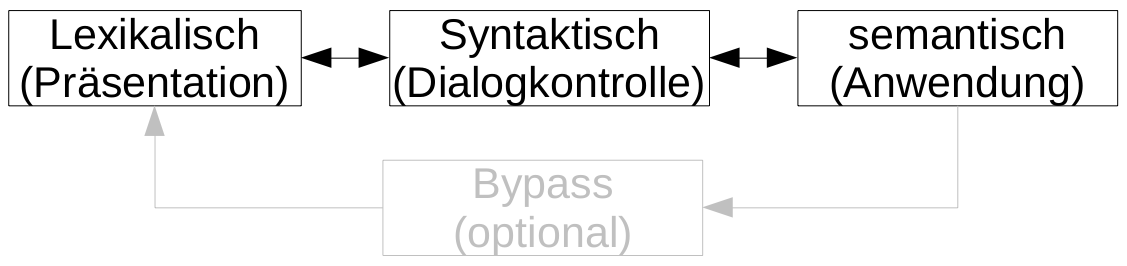
\includegraphics[width=0.4\textwidth]{Seeheim}

\minisec{PAC:}
hierarchische Elemente, jedes mit eigener Presentation, Abstraction, Control (unabhängig); \\
Vorteil: Multithreading einfach, Nachteil: Overhead    \\
\tab 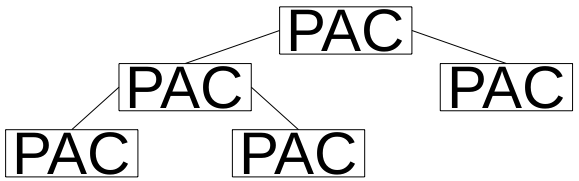
\includegraphics[width=0.3\textwidth]{PAC} \\ \\ 

\minisec{MVC:}
Model(Datenhaltung+Geschäftslogik) - View(Darstellung) - Control(Steuerung)\\
Vorteil: Model ohne View leicht testbar, Mehrere Controller einer View möglich\\
Nachteil: Mehraufwand, Trennung View-Control \\
\textbf{passive MVC:} Model reagiert auf anfragen, Kommunikation über Control\\
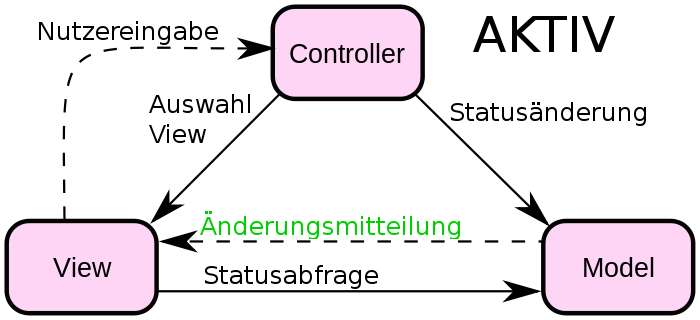
\includegraphics[width=0.25\textwidth]{aMVC} 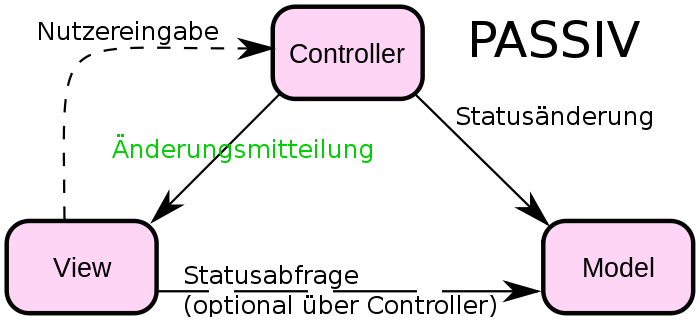
\includegraphics[width=0.25\textwidth]{pMVC} 

\textbf{Component-Based-View:} redundanzen innerhalb der View \\ $\Rightarrow$ Zerlegen in Widgets mit eigener View (evtl. auch eigene Control)


\textbf{Front-Controller:} Für Webanwendungen: leitet Anfrage an zuständigen Controller weiter


\textbf{Application-Controller:} Zusätzlicher Controller zur Verwaltung von Abhängigkeiten zwischen Seiten (reihenfolge etc.), mächtiger als Front-Controller

\minisec{Model-View-Presenter:}
Vorteile: sehr lose Kopplung der View, mehrere Presenter pro View möglich\\
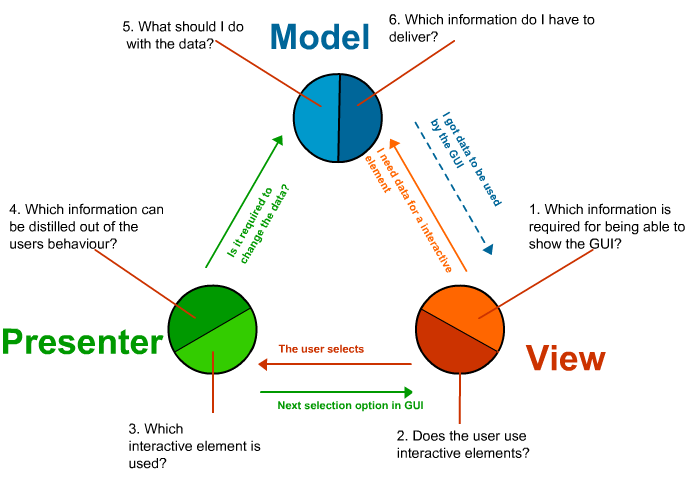
\includegraphics[height=0.46\textheight]{MVP}\\\\


\minisec{MVVM:}
Programmierer und Designer können getrennt arbeiten(XAML)\\
\oitem{View:} Umfasst XAML und Code-Behind der XAML; \\
Definition von Fenster und Widgets, UI-Interne Logik\\
\underline{Schnittstelle:} ViewModel ist DataContext der View\\
Die View bindet auf Properties und Commands des ViewModel\\
\oitem{ViewModel}: Präsentationslogik \\
Koordiniert zwischen View und Model: Konvertiert, verändert, validiert Daten\\
\underline{Schnittstelle:} Referenziert Model, \\
Implementiert Properties und Commands auf die View bindet;\\
Informiert (i.A. View) mittels Notification-Events \\
\oitem{Model}: Kapselt Daten der Anwendung und Geschäftslogik\\
sichert Konsistenz und Validität der Daten durch Geschäftslogik\\
\underline{Schnittstelle:} Keine direkte Referenz zu View/ViewModel\\ 
Änderungen im Model werden per Events signalisiert\\
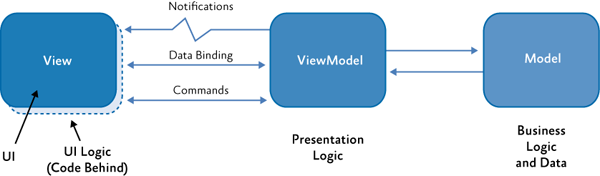
\includegraphics[width=0.5\textwidth]{MVVM}




